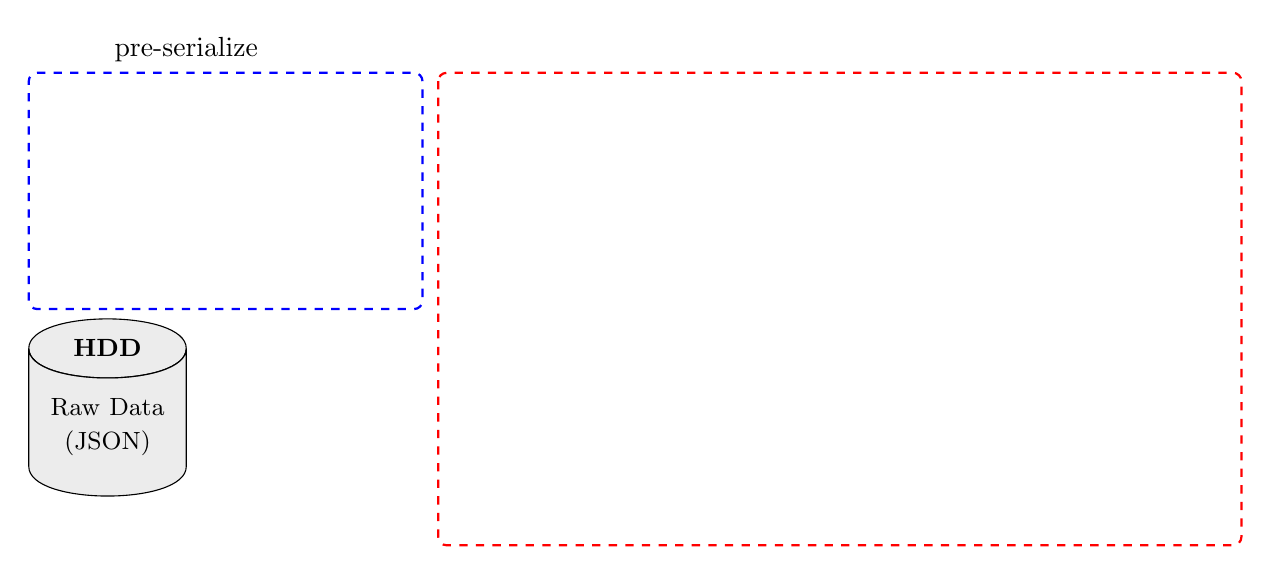
\begin{tikzpicture}
\draw (2,3.3) node{pre-serialize};
\draw[blue,thick,dashed,rounded corners=3pt](0,0) rectangle ++(5,3);
\draw[red,thick,dashed,rounded corners=3pt](5.2,3) rectangle ++(10.2,-6);

%\draw (0,0) -- (10,0) -- (10,4) -- (0,4) -- (0,0);

  \draw[fill=lightgray!60, fill opacity=0.5] (0,-0.5) to
 [controls=+(90:0.5) and +(90:0.5)] (2,-0.5);
 
 \draw[fill=lightgray!60, fill opacity=0.5] (0,-0.5) .. controls +(-90:0.5)
 and +(-90:0.5) .. (2,-0.5);
 
 \draw[fill=lightgray!60, fill opacity=0.5] (0,-0.5) .. controls +(-90:0.5)
 and +(-90:0.5) .. (2,-0.5)
 -- (2,-2) .. controls +(-90:0.5) and +(-90:0.5) .. (0,-2) -- (0,-0.5);
 
 \draw (1,-0.5) node[align=center,text width=1.5cm] {\centering\small\textbf{HDD}};
 \draw (1,-1.5) node[align=center,text width=1.5cm] {\centering\small{Raw Data (JSON)}};
 
 
 
\end{tikzpicture}